\chap{Changing Colors}\label{ch.colors}

\sect{Display colors}

Create a program that causes two different colors to be displayed on the
top of the Thymio robot when the front and back buttons are touched, and
two other colors to be displayed on the bottom of the robot when the
left and right buttons are touched.

{\raggedleft \hfill Program file \bu{colors.aesl}}

We need four event-actions pairs. There are four events---touching the
four buttons---and a color action is associated with each event. Note
the difference between the action blocks \blksm{action-colors-up} and
\blksm{action-colors-down}. The first block changes the color displayed
on the top of the robot, while the second changes the color on the
bottom of the robot. The block for the bottom light has two black marks
that represent the wheels and a white dot representing the support at
the front of the robot (\cref{fig.bottom}).

The program is shown in \cref{fig.colors}.

\begin{figure}
\gr{colors1}{.35}
\caption{Changing colors when a button is touched}\label{fig.colors}
\end{figure}

What colors are displayed? In the first three actions, the slider for
one color is moved to the right edge, while the sliders for the other
two colors are moved to the left edge. The colors are not mixed so these
actions display pure red, blue and green, respectively. The action
associated with the left button mixes red and green giving yellow. You
can see that the background of the block changes when the
sliders are moved and shows which color the robot will display.

Run the program \blksm{run} and touch the buttons to change the
robot's colors. \Cref{fig.front} shows the Thymio displaying red on the
top and \cref{fig.bottom} shows it displaying green on the bottom.

\exercisebox{\thechapter.1}{ Experiment with the sliders to see which
colors can be displayed. }

\trickbox[Information]{By mixing together red,
green and blue, you can make any color (\cref{fig.cube})!}

\begin{figure}
\gr{color-cubes}{.85}
\caption{The red-green-blue (RGB) color cube}\label{fig.cube}
\end{figure}


\sect{Multiple actions associated with one event}

Let us modify the program so that the lights are turned off when the
center button is touched. We need two actions to occur when a single
event---touching the center button---occurs. We can associate \emph{two}
actions with one event in an event-actions pair. After inserting the
event and the first action (the top color action), a gray outline will
appear to the right of the action:

\blkc{multiple-outline}

You can now drag and drop the bottom color action into this outline,
giving a pair with one event and two actions:\label{p.multiple}

\blkc{colors-multiple}

{\raggedleft \hfill Program file \bu{colors-multiple.aesl}}

Don't forget to click \blksmpure{run} to run the program. In the
future, we will not remind you to click this button to run a program.

\bigskip

\importantbox[Rules for event-actions pairs]{
\begin{itemize}[noitemsep,nosep,leftmargin=*]
\item When a program is run, all the event-actions pairs in the program
are run.
\item It is possible for several event-actions pairs to have the same
event as long as their parameters are different. For example, you can
have several pairs with the button event, if different sets of buttons
are required for different events.
\item If the event is exactly the same in two or more pairs, VPL will
display an error message (in area 3 in \cref{fig.vplgui}). You will not
be able to run the program as long as there are errors.
\end{itemize}
}

% No longer legal in 1.4
%
%\begin{figure}
%\centering
%    \subfigure[Changing colors when a button is touched]{
%		\label{fig.colors-a}
%		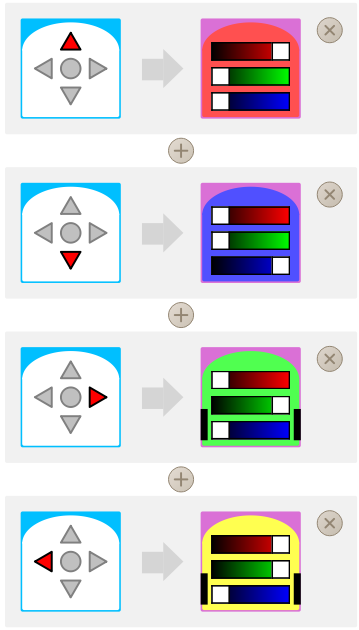
\includegraphics[width = 0.4\textwidth]{colors1}
%	}
%	\hspace{1.5cm}
%    \subfigure[Turn the colored lights off when a button is touched]{
%		\label{fig.colors-b}
%		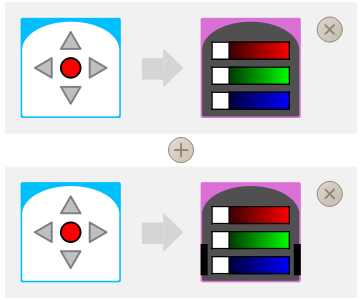
\includegraphics[width = 0.4\textwidth]{colors2}
%	}
%    \caption{Play with the lights of Thymio}
%    \label{fig.colors}
%\end{figure}
